% Desenvolvimento do projeto mobile------------------------------------------------------------------

\chapter{PORTAL ACESSÍVEL IFCE}
\label{chap:portalIFCE}
Com o conhecimento do impacto da tecnologia no ambiente educacional originou-se a ideia do Portal Acessível IFCE. Este capítulo busca detalhar a problematização encontrada no IFCE Campus Maracanaú, a solução proposta por esta pesquisa e seu processo de desenvolvimento.

\section{Campus Maracanaú}
\label{sec:campus}

%Dados iniciais de pesquisa sobre o público-alvo no Campus\\

Em uma pesquisa feita pelo instituto (\citeonline{relatorio2020}), durante um período de suspensão do calendário letivo devido à uma pandemia, tornou-se possível perceber a importância do apoio psicológico, pedagógico e social do Campus quanto aos discentes, principalmente aqueles que possuem algum tipo de deficiência. Na tabela abaixo, os dados mostram a quantidade de alunos do Campus Maracanaú que solicitaram este apoio da instituição enquanto as circunstâncias não os permitiam ter encontros e atividades letivas presenciais.

\begin{table}[!ht]
\caption{Pesquisa realizada com discentes do Campus Maracanaú}
\label{tablePesquisa}
\begin{tabular}{|l|c|}
\hline
\multicolumn{1}{|c|}{Tipo de apoio solicitado}                       & \multicolumn{1}{l|}{Quantidade de discentes} \\ \hline
Fragilidade emocional e necessidade de apoio psicológico             & 80                                           \\ \hline
Desmotivação, não se sente preparado                                 & 46                                           \\ \hline
Monitoria em algumas disciplinas, dificuldade para estudar sozinho   & 19                                           \\ \hline
Organização dos estudos, dificuldade de concentração                 & 31                                           \\ \hline
Apoio motivacional, bate-papo, trabalhos em grupo, aula motivacional & 16                                           \\ \hline
\end{tabular}
\end{table}


 
\section{O Projeto}
\label{sec:projeto}

- Explicar sobre o sistema e sobre a acessibilidade na HIG (recursos)

A \citeonline{wai2017} define que a usabilidade "é projetar produtos para serem eficazes, eficientes e satisfatórios. A usabilidade inclui design de experiência do usuário. Isso pode incluir aspectos gerais que afetam a todos e não afetam desproporcionalmente as pessoas com deficiência" (Tradução Livre).


\begin{figure}[!htb]
    \centering
    \label{fig:figura1}
    \caption{Diagrama de Casos de Uso}
    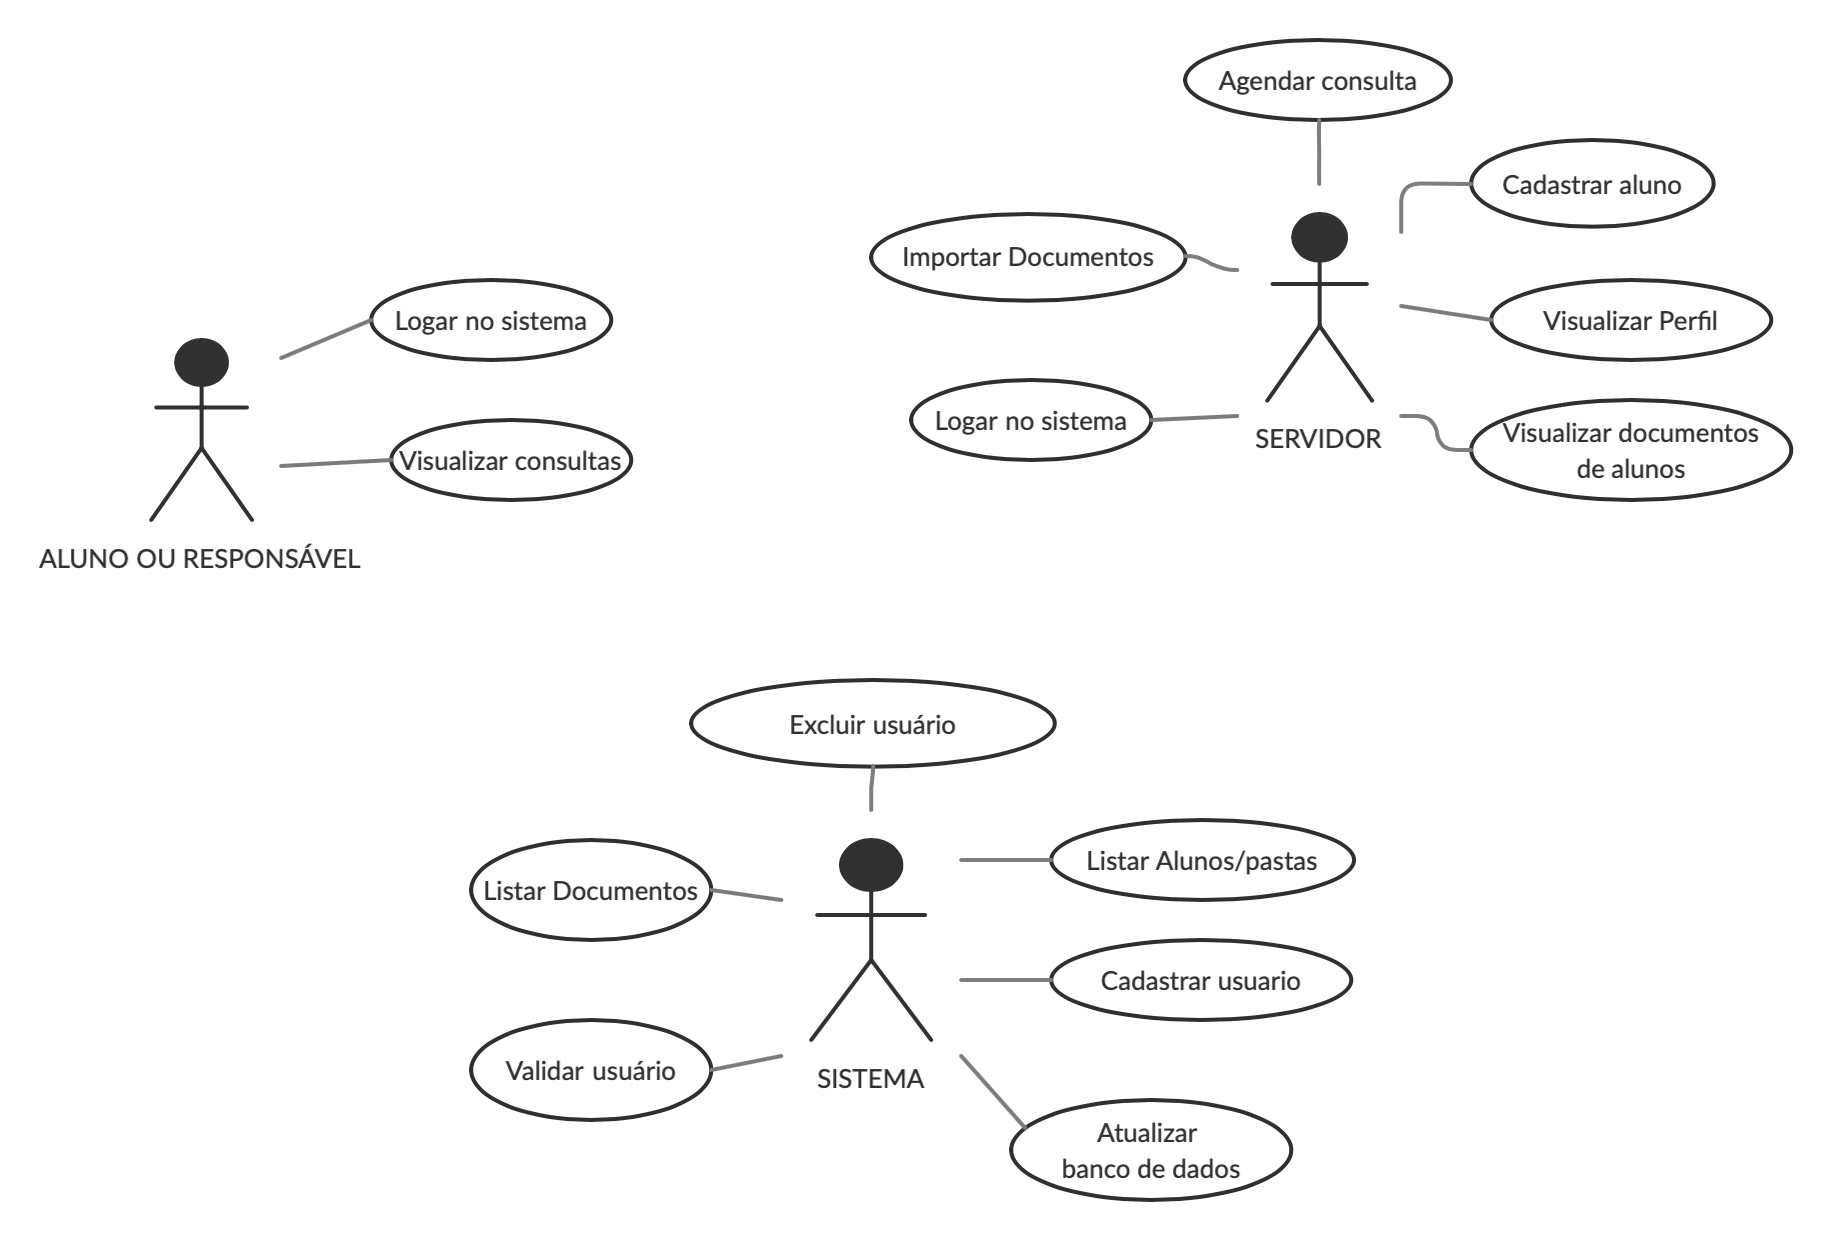
\includegraphics[width=1.0\textwidth]{./dados/figuras/Casos de uso}
    %\fonte{}
\end{figure}

\section{Levantamento de Requisitos}
\label{sec:requisitos}



%Metodologia---------------------------------------------------
\chapter{METODOLOGIA}
\label{chap:metodologia}

A fim de alcançar os objetivos propostos, a parte inicial desta pesquisa consiste em uma análise bibliográfica sobre a acessibilidade, buscando explorar experiências, regras e conhecimentos já existentes sobre o tema. 

O levantamento deste material teórico é de grande influência para a produção da ferramenta em questão tendo em vista que o projeto busca auxiliar o ambiente educacional aplicando os padrões de conteúdo acessível em um sistema para estudantes com NEE. 

Também é necessária a investigação sobre o ambiente educacional abordado pelo sistema, com informações qualitativas dos estudantes e dificuldades enfrentadas pelos profissionais do Campus. 

Para o desenvolvimento adequado do projeto, serão utilizados computadores com acesso à internet e tecnologias como:

\begin{enumerate}
    \item Kanban para gerenciamento ágil de tarefas;
    \item Linguagem de Programação Swift para o desenvolvimento da aplicação;
    \item Sketch para a etapa de prototipagem de telas;
    \item Framework XCTest para os testes unitários e de integração.
\end{enumerate}

Dentre as etapas do projeto, algumas já citadas acima, estão a etapa de Testes de UX/UI, onde os profissionais do Campus poderão opinar e expor ideias sobre a interface e o fluxo do sistema, o que guiará o design do projeto.